% Chapter1
\chapter{Einleitung} \label{chapter:introduction}

% Inhalt
% Motiviert zum Thema und führt zum Thema hin.
% Erklärt wie man löst  
% Hintergrund und Ausgangspunkt (Heutzutage statische Systeme .. Dynamik… ) Wir wollen Methoden zur Verbesserung der Anlagen ausprobieren 
% Aufgabenstellung
% Leitfaden durch die Arbeit 		

% \section{Background and Motivation} 
% \section{Objectives of this Thesis}
% Ziel dieser Abschlussarbeit
% \section{Methodology for the Developement}  
% Methoden zur Entwicklung 
% \section{Thesis Outline}
% Abschlussarbeit Gliederung

% Mehr über die statische, hardgecodete SPS'n schreiben und die das bei Änderungen sehr viel neu  gecodet werden muss -> automatische Codegenerierung. 

% Heutzutage sind Produktionsanlagen so konstruiert, dass die Reihenfolge der einzelnen Fertigungszellen fest miteinander verkettet ist. Es herrscht eine unbewegliche, statische Folge der Stationen in dem jedes Anlagemodul autark arbeitet. Wenn es bei einem Teil zu einer Störung kommt, steht der ganze Produktionsfluss ausnahmslos. Zusätzlich ist die Flexibilität der Einsatzmöglichkeit einer Produktionsanlage eingeschränkt. Neue Module in die Verkettung hinzuzufügen erfordert enorme Umbauten und Kosten. \\\\
% Weiters kommt dazu, dass der Code auf der SPS neu programmiert werden muss, wenn ein Teil der Anlage anders verwendet werden soll. Dies hat einen Stillstand der Fabrik zur Folge. \cite{lb_SFC} Allgemein sind Produktionsanlagen sehr statisch gestaltet und können nur mit viel Aufwand geändert und angepasst werden. Bei Störungen kann nur schlecht reagiert werden was wiederum fatale Ausfälle in der Produktion nach sich zieht. \cite{wlepuschitz}

%Mithilfe von einem Modell, indem die Anlage abgebildet ist, und im weiteren Schritt einer Codegenerierung . Dadurch kann ein manueller Schritt, automatisiert und dadurch auch zeit gespart werden.

% Viele Produkte auf einmal
% Individuell 
% Kurzer Lebenszyklus
% Konfigurierbar
% Hohe Qualität
% Kurze Wechsel zwischen Produkten
% Geringer Umlaufbestand 
% kundenindividuelle Massenproduktion 


%The world of industrial manufacturing faces serious challenges due to the dy- namics of the 21st century market. Even though the demand for mass com- modities remains constant or even rises as a result of growing demand from emerging economies, the continuously decreasing life cycle span of products such as mobile phones combined with an increasing individualization signifi- cantly boosts the product variety [1]. In this context, manufacturing systems are required to support mass customization with the capability of “made-to- order” instead of “made-to-stock” [2]. The concept incorporates “the ability to provide individually designed products and services to every customer through high process agility, flexibility and integration” [3]. The principle of mass customization was anticipated by Alvin To✏er already in 1970 and detailed for the first time by Stan Davis in 1987 [4]. The automotive indus- try, once prototypical for mass production, was among the earlier adopters of mass customization around 1990 with Toyota o↵ering a five-day delivery for customers, who could decide from a range of modular options concerning their desired car [5]. Even though the possibilities and conceptual aspects were already described before the turn of the millenium, the importance of mass customization as a major manufacturing strategy in various domains ranging from the food industry to mobile phones emerged only during the last decade, thereby introducing new technological demands and challenges [6]. Put in a nutshell, production systems are forced to “produce a number of di↵erent, high-quality products via short production runs, short ch times, and low work-in-process” [5].



Produktionssysteme im 21. Jahrhundert müssen wachsenden Anforderungen gerecht werden. Besonders die auftragsbezogene Einzelproduktion bringt große Herausforderung mit sich. Dabei wird eine kurze Durchlaufzeit bei hoher Qualität ebenso erwartet, sowie keine oder nur geringe Mehrkosten gegenüber der herkömmlichen Serien- und Massenproduktion. Eine Produktionsanlage muss daher unterschiedliche, hoch konfigurierbare, Produkte auf einmal schaffen können. Zusätzlich haben sich Lebenszyklen von Waren verringert, welches ein schnelles umstellen der Produktionssysteme fordert.\cite{wlepuschitz_2014} \\
Diese hohe Flexibilität hat allerdings ihren Preis. Vielfach ist es so, dass bei Änderungen wie dem Hinzufügen oder Entfernen von Teilen großer Aufwand nötig ist, um das System in neuer Zusammensetzung in Betrieb zu setzen. Besonders für die Steuereinheiten von Produktionsanlagen, die sog. speicherprogrammierbare Steuerung (SPS), muss ein Großteil des Programm-Codes neu implementiert werden. \cite{Lepuschitz_PhaseAgent}
Das Diplomprojekt hat sich zur Aufgabe gemacht, diesen Prozess näher zu untersuchen und zu klären in welchem Ausmaß und in welcher Art und Weise sich dieser Schritt anhand einer Demoimplementierung auf einer Laboranlage automatisieren lässt. 
\\\\ 
Diese Problematik der Automatisierung wird in den nächsten Abschnitten weiter beleuchtet. Dabei wird auf Motivation und Hintergrund der Arbeit eingegangen und der Stand der bereits realisierten Projekte erläutert. Ein Überblick über die Aufgabenstellung sowie ein Leitfaden durch die Arbeit schließen dieses Kapitel ab. 
\section{Hintergrund und Ausgangspunkt}
Der Verein Practical Robotics Institute Austria, kurz PRIA, dient der Förderung des wissenschaftlich-technischen Nachwuchses durch Robotik und nimmt sich der Forschungsaufgaben in verwandten Fachgebieten der Robotik und Automation an.
Im Rahmen diese Instituts wird in dem Projekt "Batch Process Automation with an On\-to\-lo\-gy-driven Multi-Agent System (BatMAS)", das von der österreichischen Forschungsföderungsgesellschaft (FFG) gefördert wird, an einem ontologiebasierten Informationsmodell, um die Konzepte von Produktionssystemen zu beschreiben, geforscht. Anhand dieses sollen intelligente Softwarekomponenten (Agenten) eingesetzt werden, die Aufträge dynamische Zuteilung um die Produktionsdauer zu verringern und damit den Durchsatz des Systems zu erhöhen. \\\\
Das Projekt Batch\_it greift diese Ansätze auf und hat sich zum Ziel gesetzt eine modellbasierte Entwicklung der Steuerung einer Produktionsanlage umzusetzen. Hierfür wird in einem Modell eine Produktionsanlage abgebildet sein, um im weitern Schritt eine automatische Codegenerierung anhand dieses zu ermöglichen. Wenn es zu Änderungen der Produktionsanlage kommt, können diese im Modell angepasst werden und durch einen Codegenerierung der nötige Anpassungsschritt der Implementierung der SPS automatisiert werden.
\begin{figure}[h!]
		\centering
		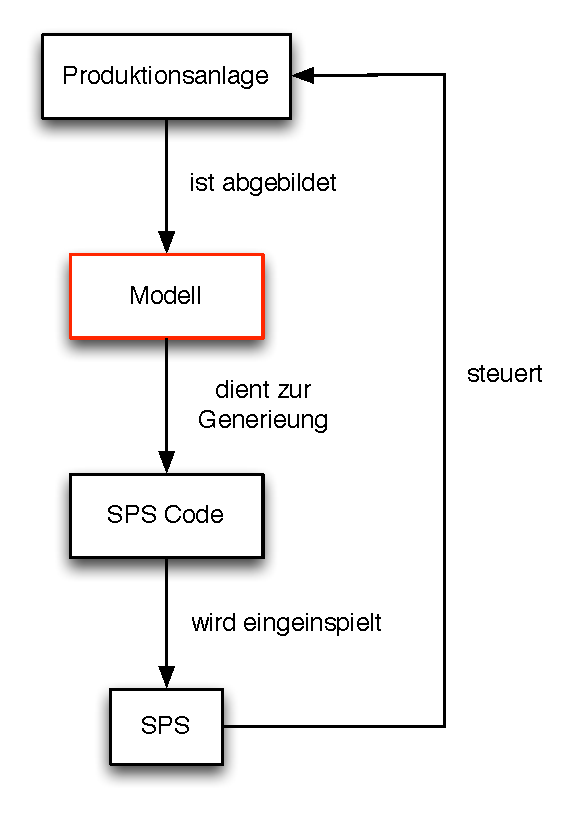
\includegraphics[width=0.49\textwidth]{graphics/ontology/konzept.pdf}
		\caption{Konzept für die modellbasierte Entwicklung der Steuerung}
		%\label{fig:MegaProxyProblem}
	\end{figure} \\
In der Abbildung 1.1 ist zu sehen, dass die Produktionsanlage in dem Modell abgebildet ist, aus dem der SPS Code generiert wird. Daraufhin kann dieser in die SPS eingespielt werden und im weitern die Anlage gesteuert werden.

%HSteuerungsaktivitäten und -funktionen, die es ermöglichen, endliche Mengen von Einsatzstoffen zu verarbeiten, indem diese unter Nutzung einer oder mehrerer Einrichtungen innerhalb eines endlichen Zeitraums einer geordneten

%Wir werden uns auf ist eine Norm für die chargenorientierte Fahrweise (Batch Control), die häufig als S88 oder SP88 bezeichnet wird. Sie ist eine Designphilosophie für Software, Ausrüstung und den Verfahrensablauf. 	



\section{Aufgabenstellung}
 Im Rahmen des Projekts Batch\_it soll eine Visualisierung und Steuerung sowie eine modellbasierte Entwicklung der Steuerung für eine Laboranlage für Chargenprozesse, die sich durch einen chargenorientierte Fahrweise (Batch Control) kennzeichnet,  implementiert werden. Dies umfasst das Erstellen von Phases nach dem IEC 61512 Standard. Hierbei handelt es sich um Funktionen wie zB. das Pumpen von Flüssigkeiten von Tank zu Reaktor oder das Heizen bzw. das Vermengen einer Flüssigkeit. Darüber hinaus werden daraus Rezepte nach dem IEC 61512 Standard entwickelt. Zusätzlich werden Fehlerszenarien einer Produktionsanlage aufgestellt, die zur spätere Entwicklung einer Fehleranalysen, dienen. Im weitern Schritt wird eine Ontologie, welche das Modell darstellt, für die Abbildung der Anlage erstellt. Anhand dieser wird eine automatische Codegenerierung für die Steuerung der Anlage implementiert.

\section{Leitfaden durch die Arbeit}
TODO
